\section{Durchführung und Aufbau}
\label{sec:Durchführung}

In Abbildung \ref{img:LIV} sieht man den verwendeten modular aufgebauten Lock-In-Verstärker.
\begin{figure}[H]
	\centering
	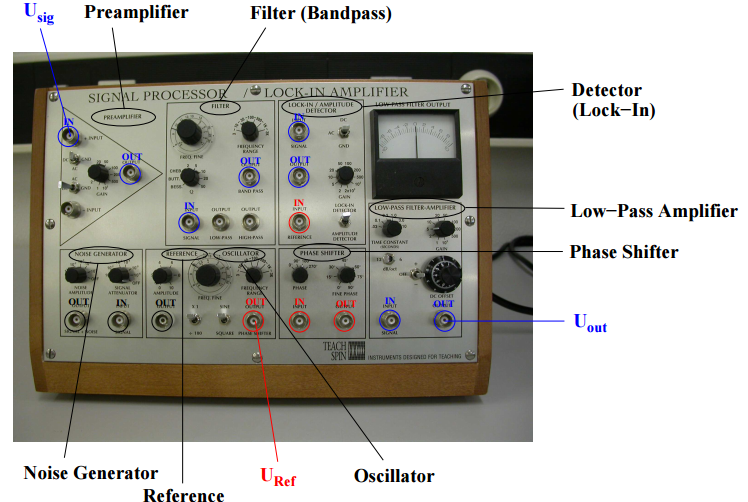
\includegraphics[height=9cm]{picture/LIV.png}
	\caption{Im Versuch verwendeter Lock-In-Verstärker. \cite[3]{sample}}
  \label{img:LIV}
\end{figure}
Im folgenden werden die einzelnen Module kurz erklärt:
\begin{itemize}
	\item Der Preamplifier verstärkt das eingehende Signal.
	\item Der Filter (Bandpass) filtert höhere und niedrigere Frequenzen aus dem Nutzsignal.
	\item Mit dem Detector werden die Signal- und die Referenzspannung multipliziert und verstärkt.
	\item Mit dem Phase Shifter wir die Phasenverschiebung zwischen Signal- und Referenzspannung eingestellt.
	\item Der Noise Generator kann ein Störgeräusch zu dem Nutzsignal hinzufügen.
	\item Das Modul Reference / Oscillator erzeugt das Nutz- und das Referenzsignal mit der Frequenz $\omega_\text{0}$.
	\item Der Low-Pass Filter / Amplifier gibt $U_\text{out}$ aus und kann dieses noch verstärken.
\end{itemize}
\newpage

\subsection{Teilversuch 1}

\begin{figure}
	\centering
	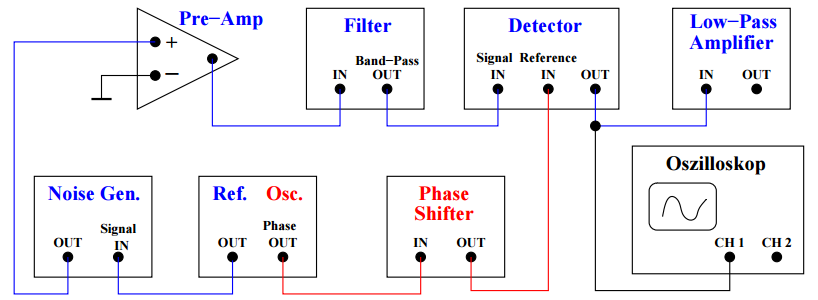
\includegraphics[height=5cm]{picture/Aufbau-Versuch1.png}
	\caption{Schaltung für den ersten Versuch. \cite[4]{sample}}
  \label{img:V1}
\end{figure}

\subsection{Photodetektorschaltung}

\begin{figure}
	\centering
	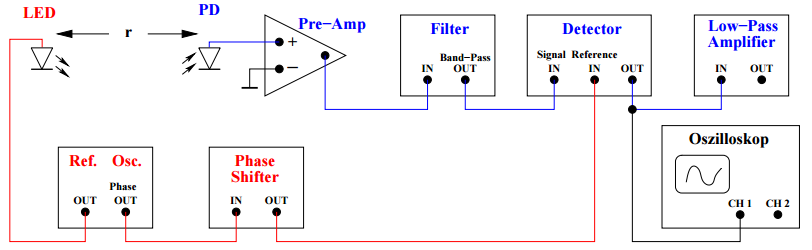
\includegraphics[height=4.5cm]{picture/Photodetektorschaltung.png}
	\caption{Die Photodetektorschaltung. \cite[5]{sample}}
  \label{img:V2}
\end{figure}
